\documentclass[english, twocolumn]{article}

%% Packages
\usepackage{amsmath}
\usepackage{amssymb}
\usepackage[hidelinks]{hyperref}
\usepackage{cleveref}
\setlength{\columnsep}{1.0cm}
\usepackage{babel}
\usepackage{color}
\usepackage{graphicx}
\usepackage{tabularx}
\usepackage{multirow}
\usepackage{diagbox}
\usepackage{array, makecell}
\graphicspath{{./figures/}}
%\usepackage[backend=bibtex,sorting=ynt,hyperref=true,backref=true]{biblatex}

\usepackage[backend=bibtex,style=numeric,sorting=nyt]{biblatex}
\addbibresource{ref.bib}
% \usepackage{breakurl}

% \makeatletter
% \usepackage{array, makecell}

%% Colors
%% - Reds
\definecolor{maroon}{RGB}{205,92,92}
\definecolor{indianred}{RGB}{128, 0, 0}
\definecolor{lightcoral}{RGB}{240, 128, 128}
\definecolor{lightsalmon}{RGB}{250, 128, 114}
\definecolor{salmon}{RGB}{233, 150, 122}
\definecolor{darksalmon}{RGB}{255, 160, 122}
\definecolor{hotpink}{RGB}{255, 105, 180}
\definecolor{brick}{RGB}{132, 31, 39}

%% - Blues
\definecolor{navy}{RGB}{0, 0, 128}
\definecolor{teal}{RGB}{0, 128, 128}
\definecolor{mauve}{rgb}{0.58,0,0.82}
\definecolor{purple}{RGB}{128, 0, 128}

%% - Greens
\definecolor{green}{RGB}{128, 128, 0}
\definecolor{olive}{RGB}{0, 128, 0}
\definecolor{dkgreen}{rgb}{0,0.6,0}

%% - Grays
\definecolor{gray}{rgb}{0.5,0.5,0.5}
\newcommand{\brokenref}[1]{\textcolor{red}{\bf#1}}
\newcommand{\raz}[1]{\textcolor{blue}{\bf#1}}
\newcommand{\mich}[1]{\textcolor{green}{\bf#1}}
% \newcommand{\ref}{\textcolor{navy}{REF}}

\title{Estimating QoE from encrypted video conferencing traffic}

\author{
    Michael Sidorov\\
    School of Electrical and\\Computer Engineering\\Ben Gurion University of the Negev\\Be'er Sheba, Israel\\
    \texttt{sidorov@post.bgu.ac.il}
    \and
    Raz, Birman\\
    School of Electrical and\\Computer Engineering\\Ben Gurion University of the Negev\\Be'er Sheba, Israel\\
    \texttt{birmanr@post.bgu.ac.il}
    \and
    Ofer Hadar\\
    Senior Member, IEEE\\School of Electrical and\\Computer Engineering\\Ben Gurion University of the Negev\\Be'er Sheba, Israel\\
    \texttt{hadar@bgu.ac.il}
    \and
    Amit Dvir\\
    Center for Cyber Technology\\Department of computer Science\\Ariel University\\Israel\\
    \texttt{amitdv@g.ariel.ac.il}
    % \date{}
}



\begin{document}


\maketitle
\begin{abstract}
Traffic encryption has become commonplace in communication over the internet, due to the threats which lurk there for unprotected "surfers". 
Though aiding security, traffic encryption renders the analytical applications that rely on clear text, and provide the means to optimize video delivery, useless. 
One such group of applications is the ones that try to estimate the Quality of Experience (QoE) of the users who consume video content. 
% Video traffic consistently, and at a high pace, becoming one of the main content categories propagated over the internet, so it is not surprising that video content providers (VCP) put much emphasis on the development of automated tools that will be able to predict QoE of the end users. 
As the demand for Video Conferencing (VC) solutions surging over the past few years,
% \cite{chang2021can} \cite{feldmann2020lockdown}
it's becoming more than ever relevant to provide a reliable QoE assessment tool also for this domain.
% and specifically for the Zoom VC application, as it was widely adapted by many schools and organizations worldwide \cite{choi2022zoom} \cite{espin2021impact} \cite{nistico2020comparative}.
Many models for QoE prediction have been proposed over the years, but most of them had two main drawbacks, viz. they dealt only with the problem of streaming video and operated mainly in an unencrypted setting, i.e., where the original image is available and can serve as a reference.
In this paper, we propose a new model for prediction of the QoE which can assess it in video conferencing applications. We developed a custom Deep Neural Network architecture, which can predict resolution, frames per second (FPS), and Naturalness Image Quality Evaluator (NIQE) criteria with an accuracy of 90.489\%, 92.492\%, and 97.643\% respectively, only from features which may be easily extracted from an encrypted traffic. The code for the network may be found at \url{https://github.com/mchlsdrv/qoe}.


% As we move forward with the development of the internet technologies, more and more threats to the end user using it arrive. Thus, it is not surprising that today the traffic encryption has become one of the basic requirements of any application using the internet. Though aiding user's security, encrypting the traffic may render the course of execution of other services difficult or even impossible. One class of  the ones which analyze the quality of experience (QoE) that the user gets from a video conferencing service (e.g., Zoom), and try to adjust various network parameters to increase it. As the demand for video conferencing services grow constantly and with a high pace, there is a great importance in being able to improve the QoE of users, and in the light of the aforementioned problem, it must be done even if all we have at our disposal is an encrypted traffic. Many efforts were applied to solve this challenge in the field of the video on demand (VoD) services. Surprisingly enough though, the venue of video conferencing (VC) has been left overlooked, which makes us, to the best of our knowledge, the first to try to address this issue here. In this paper, we study the network behaviour of an encrypted Zoom traffic, and apply several machine learning (ML) algorithms, including decision trees (DT) and neural networks (NN), to gain insight into the QoE of the end users. We find that by applying our methods, we can predict the Naturalness Image Quality Evaluator (NIQE) criterion and the frames per second (FPS) parameter, with an accuracy of 97\%, and 87\% accordingly. In addition we obtained a 76\% accuracy on the spatial frame resolution (SFR) prediction task, which stands on par with the state-of-the-art (SOTA) methods for VoD traffic prediction.
% Encryption of Internet traffic is on the rise, with transport encryption becoming a mandatory for Internet applications. While enhancing security, encryption of traffic may impede the operation of ancillary services reliant upon it. For instance, services tasked with assessing the Quality of Experience (QoE) of video conferencing platforms users, such as Zoom, may encounter difficulties in adjusting network parameters to optimize QoE. Given the persistent and rapid growth in demand for video conferencing services, there is a need to enhance user QoE, necessitating solutions that cope with encrypted traffic. While considerable efforts have been invested to address similar challenges in video on demand (VoD) services, the domain of video conferencing (VC) has been comparatively neglected, making this research, to the best of our knowledge, pioneering. In this study, we examine the network behavior of encrypted Zoom traffic and employ various machine learning (ML) algorithms, including decision trees (DT) and neural networks (NN), to gain insights into end-user QoE. We use packet measurement metrics to predict the Naturalness Image Quality Evaluator (NIQE) criterion and frames per second (FPS) parameter with accuracies of 97\% and 87\%, respectively. Furthermore, we achieve a 76\% accuracy in predicting spatial frame resolution (SFR), a performance on par with state-of-the-art (SOTA) methods for VoD traffic prediction.

% Network traffic is increasingly becoming encrypted. It is no longer possible to intercept protocol packets and derive valuable insights regarding the content. Internet users are gradually but consistently shifting their usage to video content, therefore, gaining insight into perceived Quality of Experience (QoE) of video is of a special interest. The majority of the efforts have been invested in extracting quality metrics of encrypted Video on Demand (VOD) services. However, to the best of our knowledge, no research has been reported on the use of Machine Learning (ML) for extracting quality metrics of video conferencing, also sometimes referred to as real-time video traffic. In this paper, we study the network behavior of Zoom video conferencing traffic, extract features from the encrypted network data packet streams and classify them by learning to infer Full Reference (FR) and No Reference (NR) video quality metrics. We created a dataset and trained Machine Learning (ML) models to classify the traffic quality metrics. We demonstrate an outstanding accuracy of 97\% in predicting the Naturalness Image Quality Evaluator (NIQE), and 87\% in predicting the fps. We also predicted the spatial frame resolution and obtained a 76\% accuracy level, which is consistent with the accuracy levels achieved in the state-of-the-art for VOD traffic.
\end{abstract}

\section{Introduction}
%% Version 1 (Score 100)
As we witness a significant growth of video content consumption on the internet over the past two decades, the ability to assess the QoE of the end user is becoming critical.


% Video content, rightfully, has become one of the predominant resources on the Internet over the past few years.
% As the quality of the streamed video is highly dependant on the channel it is being transmitted on, the Internet Service Providers (ISPs) are in an unique position to influence it directly, e.g., by increasing the the Band Width (BW), cache video content on servers on the Content Delivery Network (CDN), etc.

% Traffic manipulation by the ISP is usually done with tools that analyze the quality of the transferred data through a Deep Packet Inspection (DPI) tools, e.g., Wireshark, and apply traffic-enhancing algorithms to enhance the QoE of the end users. 
%% Version 1 (Score 100)
As the data communication channel plays an integral role in the final video quality, Internet Service Providers (ISPs) are placed in a unique position of being able to influence it directly, e.g., by temporarily increasing the bandwidth of a "content-hungry" network segments, or by caching the data on a Content Delivery Networks (CDNs), etc.

As most of the video content is streamed over an end-to-end encrypted channels, this procedure becoming increasingly more challenging for the ISP. While the Video Content Providers (VCP) may derive the quality of the streamed video fairly easily, e.g., by directly comparing the original image to the image which is presented to the end user, this procedure is not as straight forward to ISPs, as all they have access to is the metrics of the channel, which thought has a some indirect connection to the data streamed over it, but it is not clear how the observed metrics such as BW, latency and packet size can be related to the QoE of the end user, or even the image quality of the video.

This situation is further complected as users usually have more than a one application that requires data being transmitted over the internet. If we will add to this, the fact that in most cases data channels governed by the ISPs carry traffic which corresponds to multiple users, this problem complicates even folds more.

After the pandemic of 2019, VC application use surged \cite{chang2021can} \cite{feldmann2020lockdown}, and due to the wide adaption by many schools and organizations worldwide \cite{choi2022zoom} \cite{espin2021impact} \cite{nistico2020comparative}, QoE assessment in this domain remains a "hot" topic today.
% it's becoming more than ever relevant to provide a reliable QoE assessment tool also for this domain.
% and specifically for the Zoom VC application, as it was widely adapted by many schools and organizations worldwide \cite{choi2022zoom} \cite{espin2021impact} \cite{nistico2020comparative}.
% streams of many users is steamed over the same channel, 


% and along with this surge in demand, increases the need for Internet Service Providers (ISPs) to be able to analyze this traffic, which may be affected by a variety of factors (e.g., bandwidth, latency, packet size, etc.) 

% A large variety of traffic-enhancing algorithms and services are then applied to guarantee a good Quality of Experience (QoE). 

% Just to name a few of the services referred to above, some algorithms are designed to prioritize Voice over IP (VoIP), or services that cache the content on servers that are located closer to the end user, and by doing this, they reduce the delays in data traffic.

% Techniques for traffic manipulation, which use Deep Packet Inspection (DPI) tools, e.g., Wireshark, rely heavily on the ability of ISPs being able to analyze the data transmitted over the network. This process has become quite challenging in light of the increasing popularity of traffic encryption techniques employed in the network today, which prevents ISPs from their ability to guarantee to the end user an optimal QoE.

Though the term "good QoE" may be perceived by each individual on an intuitive level, as it is plausible to suppose that each person, if asked to rate a video, would be able to do it, it is hard to come up with a clear and objective definition to what criteria made the same person decide on the QoE of some particular video or image, as this decision usually hinges on the subjective judgment of the person asked. 

Nevertheless, we still may try to come up with a set of features that we call Key Performance Indicators (KPIs), that may exert influence when one evaluates a video. The most intuitive KPIs to recon on, are the technical ones (e.g., initial startup delay, number and duration of stalling events, and KPIs related to the image quality, viz. bit rate, and resolution.) Unfortunately, there are also quite a few features that have a less straightforward definition. Just to name a few of these are the context of the judgment (i.e., we require a higher quality presented on a higher quality monitor, or we would be less judgmental of an image of a lesser quality that is streamed over a mobile device, etc.), viewers attention to details, or even its emotional state, all may affect its final decision. 

Criteria that try to evaluate the QoE of some videos generally may be categorized into two classes, viz. Subjective and Objective. The main difference between the two classes may be summed up as the amount of human participation in the process of scoring. While criteria that correspond to the former category require full human involvement to acquire the rating, criteria that fall into the latter category can do without it.
 
One of the most widely used subjective criteria of QoE is the Mean Opinion Score (MOS), which was presented by ITU-T Focus Group on IPTV \cite{recommendation20081080}, and represents the overall acceptability of an application (or a service), perceived by the end user. It is calculated by averaging the scores assigned by participants (usually on a scale of five points) to video samples, which are designed to simulate a certain quality.

Objective criteria for QoE evaluation may be further divided into three subcategories, viz. full reference, reduced reference, and no reference, where the main difference between the three categories is the use of the original image in the evaluation process. While criteria that may be assigned to the first category use the original image as a reference to evaluate the corrupted image, criteria in the second category try to mitigate this dependence by using only the most important and easily acquired subset of features that may be used to predict the QoE. Criteria that fall into the last category go even further, i.e., they are completely independent of the original image.
% Video content, rightfully, has become one of the predominant resources in the internet over the past few years, and along with this surge in demand, increases the need of the Internet Service Providers (ISPs) to be able to analyze this traffic, which may be effected by a variety of factors (e.g., bandwidth, latency, packet size etc.) A large variety of traffic enhancing algorithms, and services are then applied to guarantee a good Quality of Experience (QoE). Just to name a few of the services referred above, there are algorithms which are designed to prioritize Voice over IP (VoIP), or services which cache the content on servers which are located closer to the end user, and by doing this, they reduce the delays in data traffic etc.
% Techniques for traffic manipulation, which use the Deep Packet Inspection (DPI) tools, e.g., wireshark, rely heavily on the ability of the ISPs being able to analyze the data transmitted in the network. This process has become quite challenging in the light of the increasing popularity of traffic encryption techniques employed in the network today, which prevents the ISPs of their ability to guarantee to the end user an optimal QoE.
% Though the term "good QoE" may be perceived by each individual on an intuitive level (as we all know what we expect from a good quality video), it is hard to come up with a clear and objective definition to what exactly it means, due to its heavy dependence on a large variety of factors, which not always objective. The most obvious, and also the easiest to recon on, are the technical ones, e.g, resolution, bit rate, delay between frames or the corruption of the image. Unfortunately, there are also quite a few features which have a less straight forward definition. Just to name a few, the context of the judgment (i.e., we require a higher quality presented on a higher quality monitor, or we would be less judgmental of an image of a lesser quality which is streamed over a mobile device etc.), viewers attention to details, or even its emotional state may affect its final decision. 
% One criterion which try to measure the QoE and assign a numeric value which represents it is the Mean Opinion Score (MOS), which was presented by ITU-T Focus Group on IPTV \cite{recommendation20081080}, and represents the overall acceptability of an application (or a service), perceived by the end user. It is calculated via averaging the scores assigned by participants (usually on a scale of five points) to video samples, which are designed to simulate a certain quality.



% Video is becoming the predominant Internet content. In the past, Internet Service Providers (ISPs) could monitor video quality in transit and apply various added value services to improve end-users' experience. For example, they prioritized multi-media content such as VoIP due to its sensitivity to real-time communication. Another example is edge caching, which brings the content closer to the subscriber in terms of network proximity, thus reducing network delays and bottlenecks. These operations were possible with Deep Packet Inspection (DPI) tools. However, today, most Internet content, including streaming video, is encrypted; therefore, ISPs had lost their ability to inspect the content, extract insights related to users experience and subsequently improve it.
% Video quality is impacted by multiple factors, including available network bandwidth and latency, devices and applications. According to the ITU-T Focus Group on IPTV ‎\cite{recommendation20081080}, QoE refers to the overall acceptability of an application or service, as perceived subjectively by the end-user. Assessment of video quality is subjective and depends on the viewer. Mean Opinion Score (MOS) is one of the well-known QoE metrics. It is based on observation and subjective classification by individual human viewers.
% Assessing the quality of encrypted video content is a challenge that has been researched in recent years. The primary focus had been Video on Demand (VOD) services such as YouTube, Netflix, Hulu, Amazon video, and the like ‎\cite{loh2020uplink}‎\cite{wassermann2019let}. These streaming video services use TCP, UDP, and in recent years QUIC transport protocols ‎‎\cite{langley2017quic}. 
% The Covid-19 pandemic has caused a significant rise in remote collaboration and the use of video conferencing as the primary mean of communication for business, education, and leisure purposes. The dominant video conferencing applications are Zoom, Microsoft Teams, and Google GoToMeeting; amongst them, Zoom conferencing is the most dominant application of choice ‎‎\cite{resources_owllabs}. 
% Several calculated QoE metrics can be extracted from video conferencing sessions to provide a meaningful representation of the Human Visual System (HVS). One of them is the VMAF ‎‎\cite{vmaf2018} (Video Multimethod Assessment Fusion) framework. VMAF is a full reference video quality estimation metric proposed by Netflix. It is considered a good QoE estimation compared to Mean Opinion Score (MOS) ‎\cite{li2018vmaf}.
% Quantization is used in lossy video compression algorithms. In compressed video streams, the Discrete Cosine Transform (DCT) block residuals are quantized such that higher spatial frequencies are zeroed up. The quantization parameter (Qp) of compressed video may be a good indication of video quality, assuming that we can estimate its value on a per frame basis from the encrypted network stream. To the best of our knowledge, this is the first research work to extract QoE of encrypted video conferencing traffic and Zoom in particular. 
% The main contribution of this paper is the inferencing of NIQE, fps, and spatial resolution QoE metrics of encrypted Zoom conferencing traffic. As a byproduct of this research work, we have also: 1) Explained observation of the unique Zoom network behavior patterns; 2) Extract low-level features from Zoom network encrypted traffic protocols to estimate the QoE according to a set of pre-defined labels. 3) Study the variation of Qp during a Zoom conference call.

\section{Related Work}

%% Version 1 (Score 100)
There are three main lines of previous work on predicting QoE from encrypted traffic, viz. methods based on statistical analysis, Machine Learning (ML) algorithms, which mainly use decision trees or their variations, and Deep Learning (DL) algorithms employing Artificial Neural Networks (ANN). 

% A large pool of work was done by now to solve the outlined problem. Previous work on predicting QoE from encrypted traffic may be divided into three lines, viz. methods based on statistical analysis, classical Machine Learning (ML) algorithms, and methods which use Deep Learning (DL) to solve it. 
% Some of the most influential methods which correspond to the former line of work used a tree-based algorithms to predict categorical features regarding the quality of the images streamed over to the user. 

%% (Score 100)
A model for YouTube quality estimation streamed over HTTPS with the Dynamic Adaptive Streaming over HTTP (DASH) protocol was proposed in \cite{dubin2016video}. They showed that an accurate classification of the image quality is achievable just by looking into the data bursts picked up from the channel during the YouTube session, which they were able to classify into three categories (viz. 360p, 480p, and 720p) with an accuracy of 97\%. 

%% Version 1 (score 98) 
% In \cite{gutterman2020requet} authors extended the work of \cite{dubin2016video}, where they again analyzed YouTube sessions with DASH protocol but tried to predict resolution on a higher granularity, i.e., having six states (144p, 240p, 360p, 480p, 720p and 1080p) instead of just three (360p, 480p and 720p). They trained a decision tree algorithm but showed worse prediction performance compared to \cite{dubin2016video}, with just 66\% accuracy. 

%% Version 2 (score 94)
In \cite{gutterman2020requet} authors extended the work of \cite{dubin2016video}, where they again analyzed YouTube sessions with DASH protocol but tried to predict resolution on a higher granularity, i.e., having six states (144p, 240p, 360p, 480p, 720p and 1080p) instead of just three (480p, 720p and 1080p), with two other metrics, which are specific to DASH sessions (the buffer, and video states.) They trained a decision tree algorithm, and thought scoring 92.0\% and 84.2\% for the last two metrics respectively, their performance for the resolution was significantly lower than of \cite{dubin2016video}, with just 66\% accuracy. Even when the problem was reduced to a binary prediction, with just two categories of small (144p, 240p, 360p) and large (480p, 720p, and 1080p), the accuracy of their model did not exceed 91\%.

%% Version 1 (Score 95)
% Mazhar and Shafiq in \cite{mazhar2018real} presented a method for QoE prediction of a video transmitted over an encrypted channel using a decision tree algorithm. More specifically, they predicted the rebuffering events, video quality, and startup delay, features that correlate with the QoE of users from streamed videos. Although achieving classification accuracy of 90\% for HTTPS and 85\% for QUIC traffic, their method has a low granularity, as for each parameter they use a binary class prediction, i.e., "at least one" rebuffering event in a video session, "high" or "low" video quality, and whether the video started before or after some predefined time threshold, which was set to 5 seconds in their experiments.
% In addition, their model predicts the QoE only retrospectively, i.e., on the whole video after the stream was completed, which renders their method less appropriate for real-time applications.

%% Version 2 (Score 98)
% Mazhar and Shafiq in \cite{mazhar2018real} presented a method for QoE prediction of a video transmitted over an encrypted channel using a decision tree algorithm to predict rebuffering events, video quality, and startup delay, features which all correlate with the QoE of users. Although achieving classification accuracy of 90\% for HTTPS and 85\% for QUIC traffic, their method has a low granularity, as for each parameter they use only a binary class prediction, i.e., "at least one" rebuffering event in a video session, "high" or "low" video quality, and whether the video started before or after some predefined time threshold.
% In addition, their model predicts the QoE only retrospectively, i.e., on the whole video after the stream was completed, which renders their method less appropriate for real-time applications.

%% Version 3 (Score 100)
Mazhar and Shafiq in \cite{mazhar2018real} presented a method for QoE prediction of a video transmitted over an encrypted channel using a decision tree algorithm to predict rebuffering events, video quality, and startup delay, features which all correlate with the QoE of users. Although achieving classification accuracy of 90\% for HTTPS and 85\% for QUIC traffic, their method has two significant drawbacks, viz. its low granularity, as for each parameter they use only a binary class prediction, i.e., "at least one" rebuffering event in a video session, "high" or "low" video quality, and whether the video started before or after some predefined time threshold, and inability to be used in an online setting, as their model predicts the QoE only retrospectively.

%% Version 1 (Score 97)
% Authors of \cite{orsolic2018youtube} proposed YouQ framework for QoE estimation in a live setting. They used a simple model that combine proportions of the time spent in a high resolution (viz. 1080p or 720p) and the duration of the stalling events during the video playback time. According to the computed statistics, they classify each YouTube session into one of three categories, viz. "high," "medium," and "low." The method was evaluated against the MOS of human participants. Authors performed two lines of experiments using a binary label (viz. "high" or "low") in the first and achieved 91\% accuracy that dropped to 84\% after the addition of just one extra class (viz. "medium"), which highlight the weakness of their approach.

%% Version 2 (Score 99)
% Authors of \cite{orsolic2018youtube} proposed YouQ, a framework for QoE estimation in a live setting. They used a simple model that combine proportions of the time spent in a high resolution (viz. 1080p or 720p) and the duration of the stalling events during the video playback time. They evaluated their method against the MOS of human participants. In their work, authors have conducted two lines of experiments using a binary label (viz. "high" or "low") in the first and achieved 91\% accuracy that dropped to 84\% after the addition of just one extra class (viz. "medium"), which highlight the weakness of their approach.

%% Version 3 (Score 100)
Authors of \cite{orsolic2018youtube} proposed a YouQ, a framework for live QoE estimation. They used a simple model that combine proportions of the time spent in a high resolution (viz. 1080p or 720p) and the duration of the stalling events during the video playback time. They evaluated their method against the MOS of human participants. In their work, authors have conducted two lines of experiments using a binary label (viz. "high" or "low") in the first and achieved 91\% accuracy that dropped to 84\% after the addition of just one extra class (viz. "medium"), which highlight the weakness of their approach.

%% Version 2 (Score 94)
% The model presented in \cite{bronzino2019inferring} uses features from IP stack layers (viz., Network, Transport, and Application), to train a random forest regressor to predict startup delay and resolution in a real-time setting for four video streaming services, viz. YouTube, Netflix, Amazon and Twitch. 
% They trained layer-specific and composite models, where the former used features from a single layer of the IP stack, e.g., the transport layer, while the former combined features from two different layers, e.g., Network and Transport, Network and Application, etc. Their training routine included two settings, namely an application-specific and cross-application setting. While in the first training routine, the training data was acquired from a single streaming service they used training data from multiple platforms for the second training routine.  
% Though achieving an error as small as 1 second for startup delay and precision of 93\% for the resolution prediction, neither of their models could generalize well to data from an application on which it was not trained, e.g., a model trained on data exclusively from Netflix could not perform well on test data from either of YouTube, Amazon or Twitch.

%% Version 2 (Score 98)
% Authors in \cite{bronzino2019inferring} tried to improve on the results from \cite{mazhar2018real} by extending its predictive granularity. In their experiments, they trained a random forest model on features from layers of the IP stack, extracted from video streaming sessions. Their dataset included sessions of four popular video streaming platforms, viz. YouTube, Amazon, Netflix, and Twitch. Authors showed that their method, when trained on cross-layer data, may predict video resolution with an accuracy of 93\%.

%% Version 3 (Score 100)
Authors in \cite{bronzino2019inferring} tried to improve on the results from \cite{mazhar2018real} by extending its predictive granularity. In their experiments, they trained a random forest model on features from layers of the IP stack data. Their dataset included sessions of four popular video streaming platforms, viz. YouTube, Amazon, Netflix, and Twitch. Though the proposed method predicted video resolution with an accuracy of 93\%, it could not generalize well to other datasets.

%% Version 1 (Score 93)
One of the first studies investigating the QoE in VC applications was performed by \cite{chang2021can}. The authors studied the influence of the movement in the presented frame on the QoE of the end user. They conducted 700 controlled VC sessions on three popular VC platforms (viz. Zoom, Webex, and Google Meet), in which they presented videos with high and low movement. They used standard metrics for image quality evaluation, viz. PSNR (Peak-to-Noise Ratio), SSIM (Structural Similarity Index), and VIFp (Pixel Visual Information Fidelity) to infer the QoE of the user. 
The main limitations of this work, as pointed out by the authors themselves, were the lack of generality in their experiments, i.e., they used specific settings that may not always represent the general use case. In addition, they only performed their experiments for small-sized conferencing sessions (less than 11 participants), which may not be projected on medium and large conferencing sessions directly.

% In \cite{chang2021can} the authors perform a study of user-perceived performance of zoom, Webex and Google Meet in terms of streaming lag time, bandwidth requirements, quality (PSNR, SSIM, and VIFp), computing requirements, and how they are impacted by geography. 

%% Version 1 (Score 100)
Yet another study in \cite{macmillan2021measuring} considered the VC applications, but this time investigated differences in the minimal requirements to avoid a decrease in the QoE. They performed controlled experiments in which they varied the bandwidth of the down and the uplink separately, and other modalities such as the number of participants and the viewing mode (i.e., single image of the speaker or a gallery), comparing the behavior of three popular VC applications, viz. Zoom, Google Meet, and Teams. Interestingly, the authors showed that viewing mode may reduce uplink utilization through the reduction in the resolution of the displayed image. One possible limitation of this work is its strong association with geographical location, as their entire dataset originated from the same University.
% \cite{macmillan2021measuring} Investigated the behavior of Zoom, Microsoft Teams and Google Meet VC applications and reported significant differences in network utilization, encoding strategy, and recovery time after network disruption. 

%% Version 1 (Score 100)
% As Zoom uses a proprietary header format that makes feature extraction challenging, a study in \cite{michel2022enabling} provided a method to extract packet-level features such as media bit-rate, frame size, frame rate, latency of the video stream, and jitter. 

%% Version 2 (Score 100)
As Zoom uses a proprietary header format that makes feature extraction challenging, a study in \cite{michel2022enabling} provided a method to extract packet-level features such as media bit-rate, frame size, frame rate, latency of the video stream, and jitter. 
In their work, they outline the problem of retransmission identification and propose a \textit{frame delay} metric, which they define as the time between the first packet of a frame and the end of frame transmission, which should indicate if a high number of retransmissions occur during the session.


% The paper in \cite{michel2022enabling} offers A detailed analysis of how the proprietary Zoom application layer protocol works at the packet level. The authors identify unencrypted fields in the Zoom packet format, find how to group streams into meetings, and how to identify peer-to-peer meetings. While the paper focus is on Zoom performance and behavior metrics under different network conditions, it does not infer end-user QoE. We do not focus on packet level analytics, but instead focus on predicting QoE metrics from the entire Zoom encrypted traffic stream using ML algorithms

\section{Data}
%% Version 1 (Score 100)
We evaluated the performance of our model on a custom dataset that imitated Zoom sessions under various channel bandwidths (changed with the NetLimitter application). It included network channel data pickup from 720 controlled Zoom sessions, where the features in \cref{tab:zoom-features} were collected and averaged over one second to decrease the noise.

% To test the performance of our models, we created a labeled dataset of Zoom calls, where we used the Netlimitter traffic control software to limit the bandwidth of the channel, to simulate various network conditions. The dataset contains 720 samples, where each sample is an average over the measurements over 1 sec taken while modifying channels' bandwidth.
% and for each of the samples different parameters were extracted from the encrypted traffic, e.g., bandwidth, resolution, FPS, latency etc. 
% We train ML algorithms to predict QoE metrics from encrypted Zoom video conferencing traffic. To accomplish that, we have created a dataset of labeled samples. In order to assess the Zoom video quality degradation and build a suitable dataset to predict it, we studied the behavior of the Zoom video session under changing network channel conditions. Analyzing the Zoom behavior pattern, we realized that the focus should be on the transition periods, where the spatial as well as the temporal resolutions are interchangeably affected. Each sample in our dataset is averaged over a 1 sec interval taken while modifying the channel bandwidth by the Netlimiter traffic control software. For each data sample we captured the features and the labels. Our dataset includes 720 samples and can be downloaded from https://github.com/yogevdrori/Encrypted-Zoom-traffic-dataset.git.



\subsection{Features}
Zoom provides several metrics available for the end user through its' Software Developer Kit (SDK), which may be automatically extracted from the session stream in real time. For our dataset we captured all them, as we wanted to explore their predictive ability of the QoE. All the features in our dataset are listed in \cref{tab:zoom-features}.

\begin{table*}
    \caption{Features extracted from the encrypted Zoom traffic for the dataset}
    \centering
        \begin{tabular}{l|l}
            Feature & Description \\        
            \hline
            Bandwidth & \makecell[l]{The number of bits per second allowed to be\\transmitted on the channel}\\
            Resolution & \makecell[l]{The number of pixels in the width and the\\length of the presented image}\\
            FPS & The number of frames per second in the playback\\
            Latency & Initial time after which the video starts\\
            Jitter & \makecell[l]{Statistical variance of the Real-time Transport Protocol (RTP)\cite{schulzrinne2003rfc3550}\\data packet in time interval}\\
            PPS & Number of transmitted packets in each second\\
            Destination port & \makecell[l]{The $2^{nd}$ layer port on the remote host where\\ the transmitted data is directed to}\\
            Source port & \makecell[l]{The $2^{nd}$ layer port on the local host through which\\the data is transmitted}\\
            \makecell[l]{Average time\\between packets} & \makecell[l]{The time difference between the reception of two\\consecutive packets}\\
            Packet length & Number of bytes in each transmitted packet\\
        \end{tabular} 
    \label{tab:zoom-features}
\end{table*}

\subsection{The QoE Metric}
In our experiments we used the Naturallness Image Quality Evaluator (NIQE) metric proposed \cite{mittal2012making}.  
% Just by looking at an image, or a video, we can asses its' quality fairly quickly. However finding an objective criterion for quality assessment is a challenging task for an automated system. Many lines of work tried to propose their criteria for a numeric quality measure, but all divide into two categories, viz. Full Reference (FR) and No Reference (NR) QoE metrics. The difference between the two may be summarized in the fact that while the former requires human assessment, the latter uses algorithmic approach to achieve the quality criterion. In this work we chose to concentrate on one metric from each category, i.e., the Video Multi-method Assessment Fusion (VMAF) \cite{li2016toward} as the FR QoE metric, whereas for the NR metric we chose the Naturalness Image Quality Evaluator (NIQE) \cite{mittal2012making}.

% \subsection{VMAF metric}
% This metric was developed by Netflix as an alternative to the Peak Signal-to-Noise Ratio (PSNR) metric which is defined via the Mean Squared Error (MSE) of the original image $I$ and the lossy image $L$ as is shown in \cref{eq:mse} and \cref{eq:psnr}.
 
% \begin{equation}
%     MSE[I, L] = \frac{1}{mn}\sum_{i=0}^{m-1}\sum_{j=0}^{n-1}[I(i, j) - L(i, j)]^2
%     \label{eq:mse}
% \end{equation}
% \begin{equation}
%     PSNR = 10 log_{10}(\frac{MAX_I^2}{MSE})
%     \label{eq:psnr}
% \end{equation}

% As the authors of \cite{li2016toward} maintain that PSNR does not provide a reliable criterion for the QoE assessment. They develop the VMAF as a Machine Learning (ML) based metric, which teaches a Support Vector Machine (SVM) model on three basic metrics, i.e., two for image quality, viz. Visual Information Fidelity (VIF) \cite{sheikh2006image} and the Detail Loss Metric (DLM) \cite{li2011image}, and one for temporal quality assessment, viz. Motion, which performs a simple average of absolute differences of pixel wise intensities between two consecutive frames. 

% VMAF uses as labels human assessment on video fragments corrupted with noise with the corresponding clean reference video fragment (i.e., without noise added). Human evaluators rate the corrupted video fragment on a scale of 1 to 5 (i.e., where 1 means "very annoying" while 5 is "not noticeable"). Than the scores for each video and from every evaluator are combined and normalized to form the Differential Mean Opinion Score (DMOS) which lays in the range of [0, 100], where the score of 100 given for the reference video.
% We extracted several FR video quality metrics from Zoom traffic. In order to assess the quality degradation caused by reduced bandwidths, we needed to compare a reference source video of original quality to the same video stream at the receiving end, that was impacted by the network conditions. We have access to the video that is recorded by the Zoom application. We observed that when establishing a 2-party conference call, Zoom reduces the quality of the recorded video at the source and at the destination at the same time. In order to obtain a good quality reference, we managed to force the Zoom application to produce and record a good quality video. This was accomplished by adding to the call a 3rd party without a bandwidth limitation. This way the sending Zoom application allows to record a good quality reference which is not impacted by the restricted bandwidth of the 2nd party to the call. The setup used to record the reference and the destination videos is depicted in \Cref{fig:vmaf-setup}. In order to perform a reasonably accurate comparison between the 2 recorded streams, they have to be synchronized. We used the audio recording to synchronize the streams by creating an abrupt loud instantaneous noise (similar to "cut" used in recording a movie "video take") and synchronized the videos at the sender and recipient ends using that noise.
% The results of the Full reference video QoE metrics measured using the setup depicted in \Cref{fig:vmaf-setup} are provided in \Cref{fig:qual-metrics}. The slight improvement of quality observed when the bandwidth is decreased can be explained by the slight decrease of the Qp parameter performed by Zoom during the bandwidth drop transition period (depicted in \Cref{fig:adapt-patt}). It is assumed that Zoom decreases the Qp to compensate for reduced quality during the bandwidth drop transition.

\subsection{NIQE Metric}
Due to the challenges of recording Zoom video sessions with FR and in order to make the dataset more accommodating to future expansions (which do not necessitate complicate setups and saving of a reference for each recorded video clip), we researched the No Reference (NR) QoE metric alternatives. A promising NR metric that has emerged is the Naturalness Image Quality Evaluator (NIQE) \cite{mittal2012making}, which measures the distance of the frame from naturalness, therefore, a smaller score indicates better perceptual quality. NIQE measures the distance between the Natural Scene Statistics (NSS)-based features calculated from an image to the features obtained from an image database used to train the model. The features are modeled as multidimensional Gaussian distributions. We calculated NIQE as a function of bandwidth, resolution and FPS. The corresponding graphs are depicted in \Cref{fig:niqe-fps-bw-res}. As can be seen in \Cref{fig:niqe-fps-bw-res} (b) and (c), the NIQE is consistent with available bandwidth and video frame resolution respectively, such that the larger the bandwidth or the resolution, the smaller the NIQE, thus indicating better quality.  We can observe a range of resolutions for which the NIQE value remains constant, indicating that the image naturalness metric at these resolutions is sufficiently good despite the change. An interesting observation is depicted in \Cref{fig:niqe-fps-bw-res} (a), indicating a change of NIQE with FPS, whereas the metric is measured per single frame and is therefore spatial by nature. The temporal resolution of the video frames has an impact on the spatial quality. This is due to the compression algorithm that utilizes quantized residuals which are determined by block prediction accuracy, which is in turn impacted by the magnitude of the Motion Vectors (MV) used for Inter-prediction. The larger the movement between consecutive frames, the larger the MV magnitude and the less accurate is the prediction, thus increasing the value of the temporary predicted block residuals and reducing the quality due to their quantization.

% This metric is based on the assumption that natural images (i.e., images which represent objects commonly observed in nature), and the features contained in them, may be expressed by features that follow the Multi-Variate Gaussian(MVG) \nomenclature{MVG}{Multi-Variate Gaussian} model. 

% This QoE technique expresses the image as a collection of quality-aware features, i.e., features that are derived from a simple, but highly regular Natural Scene Statistics (NSS) \nomenclature{NSS}{Natural Scene Statistics} model \cite{ruderman1993statistics} that are fitted to the MVG; an example for such a feature may be expresses as a local mean and contrast estimation with a MVG of some normalized (i.e., by removing the mean and dividing by a standard deviation of pixel values) image patch $I$, as shown in \cref{eq: niqe-feat-mu} and \cref{eq: niqe-feat-sigma}, where $\hat{I}(i,j) = \frac{I(i,j) - \mu(i,j)}{\sigma(i,j) + 1}$, and $w = \{ w_{l,k | k = -K,...,K, l = -L,...,L}\}$, which is a 2D circularly-symmetric Gaussian weighting function sampled out 3 standard deviations and rescaled to unit volume (i.e., $K=L=3$).

% \begin{equation}
%     \mu(i, j) = \sum\limits_{k=-K}^{K}\sum\limits_{l=-L}^{L}w_{k,l}\hat{I}(i+k, j+l)
%     \label{eq: niqe-feat-mu}
% \end{equation}

% \begin{equation}
%     \sigma(i, j) = \sqrt{\sum\limits_{k=-K}^{K}\sum\limits_{l=-L}^{L}w_{k,l}\left[\hat{I}(i+k, j+l) - \mu(i,j)\right]^2}
%     \label{eq: niqe-feat-sigma}
% \end{equation}

% Finlay, NIQE is expressed by the mean distance of the collection of the NSS features extracted from image patches to the NSS features extracted from the corpus of natural images

% \subsection{Labels}
% Zoom provides several metrics available for the end user through its' Software Developer Kit (SDK), which may be automatically extracted from the session stream in real time, and latter used as labels for the supervised model training. 
% The User Interface (UI) of the Zoom application provides several QoE metrics. We used the Zoom Software Developers Kit (SDK) to extract these metrics programmatically and used them as labels. The Labels that we extracted from Zoom and used as QoE metrics are latency, Jitter, Resolution, and frames per second (fps). The predominant parameters used by the Zoom application when adapting to network channel conditions are Spatial and Temporal resolutions, whereas the spatial resolution is the frame image pixels density and the temporal resolution is the frame rate, measured in frames per second (fps). The Zoom SDK screen that indicates these labels is depicted in \Cref{fig:qoe-from-app}. The application captures the quality metrics at the sending and at the receiving end. We noticed that the resolution is also impacted by the size of the video window selected by the user – in the case of a smaller video window, the resolution is reduced and in the case of a larger window, it is increased.
% In addition to the quality metrics that are extracted directly from the Zoom application, we also used additional video QoE metrics. We built a setup to capture Full Reference (FR) metrics \Cref{fig:exp-setup},  such as VMAF ‎\cite{li2018vmaf} and also implemented No Reference (NR) metrics such as NIQE ‎\cite{mittal2012making}.
\subsection{Exploratory Data Analysis (EDA)}
\label{sec:eda}
First, we performed a simple Pearson correlation \cite{pearson1895vii} of the extracted features, which is listed in \cref{tab:corr_table}. This analysis highlighted the features which influence the target (i.e., the NIQE), the most. Pearson correlation is a measure of the influence which some feature $X$ has on its' counterpart $Y$, i.e., how precisely can we anticipate a change (positive or negative) in $Y$ by observing $X$, and is defined as 

\begin{equation}
    \rho_{X,Y} = \frac{Cov[X,Y]}{\sigma(X)\sigma(Y)}
\label{eq:pearson_cor}
\end{equation}
This measure is located in the range [-1, 1], where 1 points to a perfect positive correlation, i.e., increase in one feature brings increase in the other, while -1 signifies a total reverse correlation, accordingly, which may be seen in \Cref{tab:corr_table}. Features with correlation closer to $\pm{1}$ are the most interesting, as it indicates that this feature, or it reverse, has strong effect on the predicted variable. 
Among the strongest predictive values we see \emph{bandwidth} (-0.78), \emph{resolution} (-0.73), \emph{FPS} (-0.76), \emph{average time between packets} (0.77), and surprisingly, also \emph{packet length} (-0.86). 

As for the first three, its is quite intuitive that increase in their value will decrease the NIQE, as higher bandwidth leads directly to better resolution and fps, which in its' turn improves the perceived quality of the video. 

The \emph{average time between packets}, which has a strong positive correlation with NIQE, i.e., increase in this feature leads to worse QoE of the observer (as a high NIQE means worse QoE than a low one). This is also intuitively clear, as packages which arive at a lower rate may indicate a lower FPS.

The high negative correlation of the \emph{packet length} though is less intuitive, but yet has an explanation, viz. as we increase the bandwidth, video compressor has the ability to place more data in each packet, increasing the FPS, and by this increasing also the QoE of the viewer.

In addition, to reduce the dimensionality of our dataset even further, we performed the the Primary Component Analysis (PCA) \cite{pearson1901liii} algorithm, which may be seen as a method to project the data to a lower dimensional subspace, but one that still contain most of the information from the original space. The results of this procedure are presented in \cref{fig:pca}, and in the corresponding \cref{tab:pca_loadings}.
% on the features in our dataset to acquire a subspace where the features will be sorted by their importance \Cref{fig:pca}.
From this analysis we conclude that the by transforming the features with the corresponding loadings, we can use as few as 5 features instead of the 9 original and still retain 99\% of the information present in the data.


\begin{table*}[t]
    \caption{Pearson correlation of different features in the dataset. In bold script are the features with the largest positive or negative correlation with the explained feature, i.e., NIQE}
    \centering
    \scalebox{0.8}{
        \begin{tabular}{l|c|c|c|c|c|c|c|c|c|c|c}
             & BW & NIQE & Resolution & FPS & Latency & Jitter & PPS & Destination & Source & Average time & Packet\\
             & & & & & &  & & Port & Port & between packets & Length\\
             \hline
             \textbf{BW} & 1.0 & \textbf{-0.777} & 0.586 & 0.656 & -0.274 & -0.383 & 0.946 & -0.032 & 0.056 & -0.931 & 0.873\\
             NIQE & -0.777 & 1.0 & -0.728 & -0.758 & 0.391 & 0.486 & -0.666 & 0.067 & -0.088 & 0.770 & -0.860\\
             \textbf{Resolution} & 0.586 & \textbf{-0.728} & 1.0 & 0.765 & -0.417 & -0.458 & 0.493 & -0.111 & 0.132 & -0.593 & 0.719\\
             \textbf{FPS} & 0.656 & \textbf{-0.758} & 0.765 & 1.0 & -0.478 & -0.495 & 0.591 & -0.071 & 0.094 & -0.679 & 0.693\\
             Latency & -0.274 & 0.391 & -0.417 & -0.478  & 1.0 & -0.798 & -0.231 & 0.042 & -0.061 & 0.284 & -0.359\\
             Jitter & -0.383 & 0.486 & -0.458 & -0.495  & -0.798 & 1.0 & -0.328 & 0.018 & -0.040 & 0.377 & -0.467\\
             \textbf{PPS} & 0.946 & \textbf{-0.666} & 0.493 & 0.591  & -0.231 & -0.328 & 1.0 & 0.022 & 0.004 & -0.933 & 0.721\\
             Destination Port & -0.032 & 0.067 & -0.111 & -0.071  & 0.042 & 0.018 & 0.022 & 1.0 & -0.985 & 0.012 & -0.074\\
             Source Port & 0.056 & -0.088 & 0.132 & 0.094  & -0.061 & -0.040 & 0.004 & -0.985 & 1.0 & -0.044 & 0.106\\
             \makecell[l]{\textbf{Average time}\\\textbf{between packets}} & -0.931 & \textbf{0.770} & -0.593 & -0.679  & 0.284 & 0.377 & -0.933 & 0.012 & -0.044 & 1.0 & -0.783\\
             \textbf{Packet length} & 0.873 & \textbf{-0.860} & 0.719 & 0.693  & -0.359 & -0.467 & 0.721 & -0.074 & 0.106 & -0.783 & 1.0\\
        \end{tabular}
    }
    \label{tab:corr_table}
\end{table*}

\begin{figure}
    \centering
    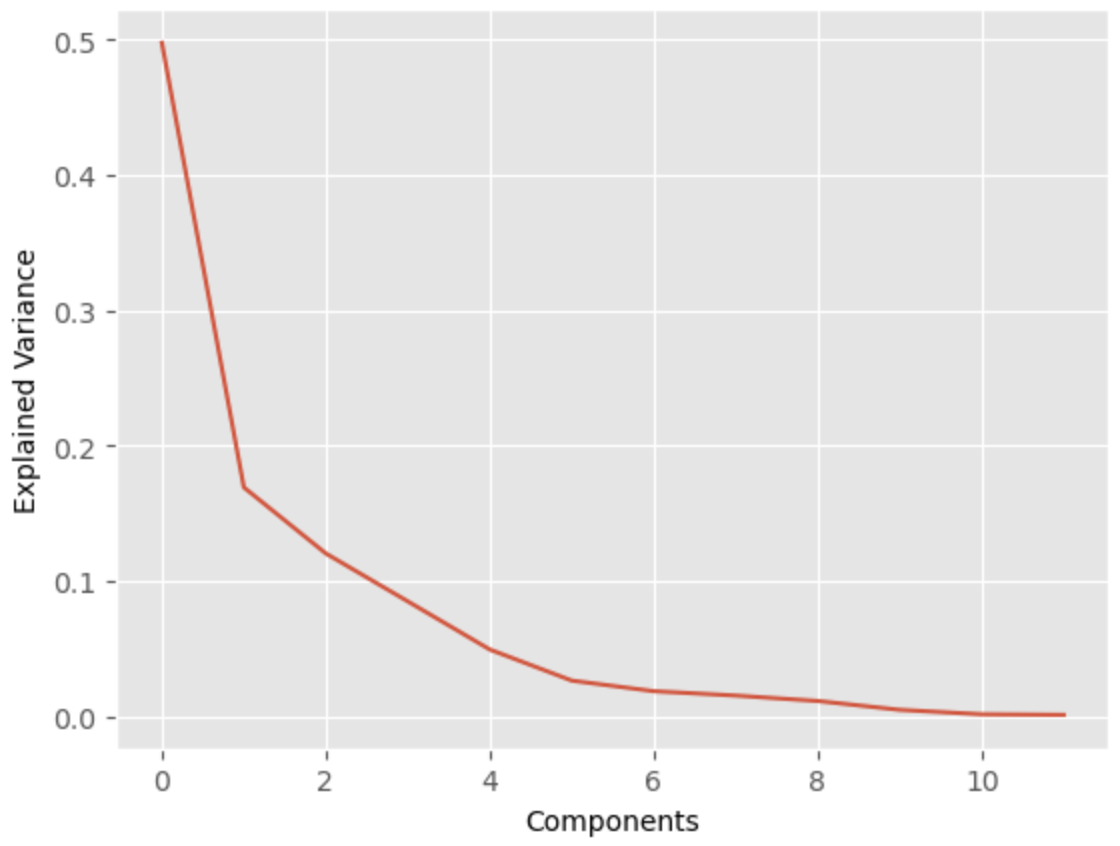
\includegraphics[scale=0.4]{pca.png}
    \caption{Primary component analysis (PCA) on the 12 features in our dataset}
    \label{fig:pca}
\end{figure}

\begin{table*}[]
    \caption{PCA loadings and the corresponding accumulative variance summation for each PC, for features with the correlation $|\rho|>0.5$, which presented in \cref{tab:corr_table}}
    \centering
    \begin{tabular}{l|c|c|c|c|c|c|c|c}
      &   PC0  &  PC1  &  PC2   &  PC3  &  PC4  &  PC5  &  PC6  &  PC7  \\
    \hline
    Bandwidth   & -0.402 & 0.277 & 0.212  & 0.116 & 0.012 & 0.126 & 0.314 & 0.767 \\
    Resolution  & -0.346 & -0.107& -0.667 &	0.201 & -0.453&	-0.411&	0.084 &	0.051 \\
    FPS	        & -0.368 & -0.097& -0.432 & -0.615& 0.495 & 0.201 &	0.071 &-0.016 \\
    Latency     & 0.236	 & 0.636 & -0.240 & 0.189 &	0.504 &	-0.439&	0.002 &-0.005 \\
    Jitter      & 0.273	 & 0.562 & -0.305 & -0.239&	-0.455&	0.502 &	-0.004&-0.014 \\
    PPS         &-0.375  & 0.321 & 0.350  & -0.215& -0.176& -0.215& 0.477 &-0.533 \\
    \makecell[l]{Avg. time\\between packets} & 0.397 & -0.263 & -0.197 & 0.193 & 0.125 & 0.171 & 0.807 & -0.032 \\
    Packets length & -0.394 & 0.102 & -0.113 & 0.626 & 0.205 & 0.504 & -0.102 & -0.351 \\
    \hline
    \hline
    Cumulative variance & 0.648 & 0.827 & 0.907 & 0.944 & 0.967 & 0.990 & 0.998 & 1.\\        

    \end{tabular}

    \label{tab:pca_loadings}
\end{table*}

\begin{figure}
    \centering
    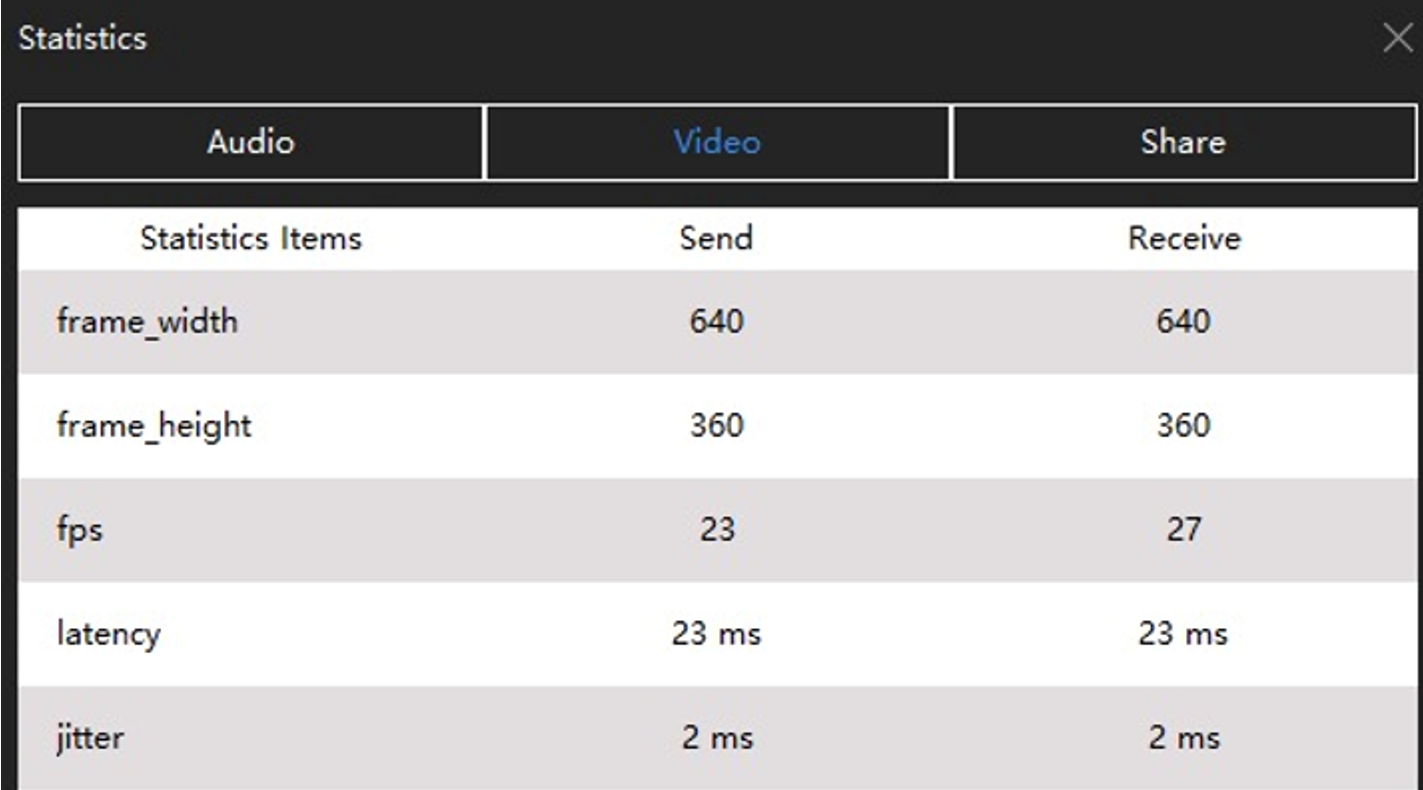
\includegraphics[scale=0.18]{data_examp.png}
    \caption{Zoom quality of experience extracted from an application}
    \label{fig:qoe-from-app}
\end{figure}

\begin{figure}
    \centering
    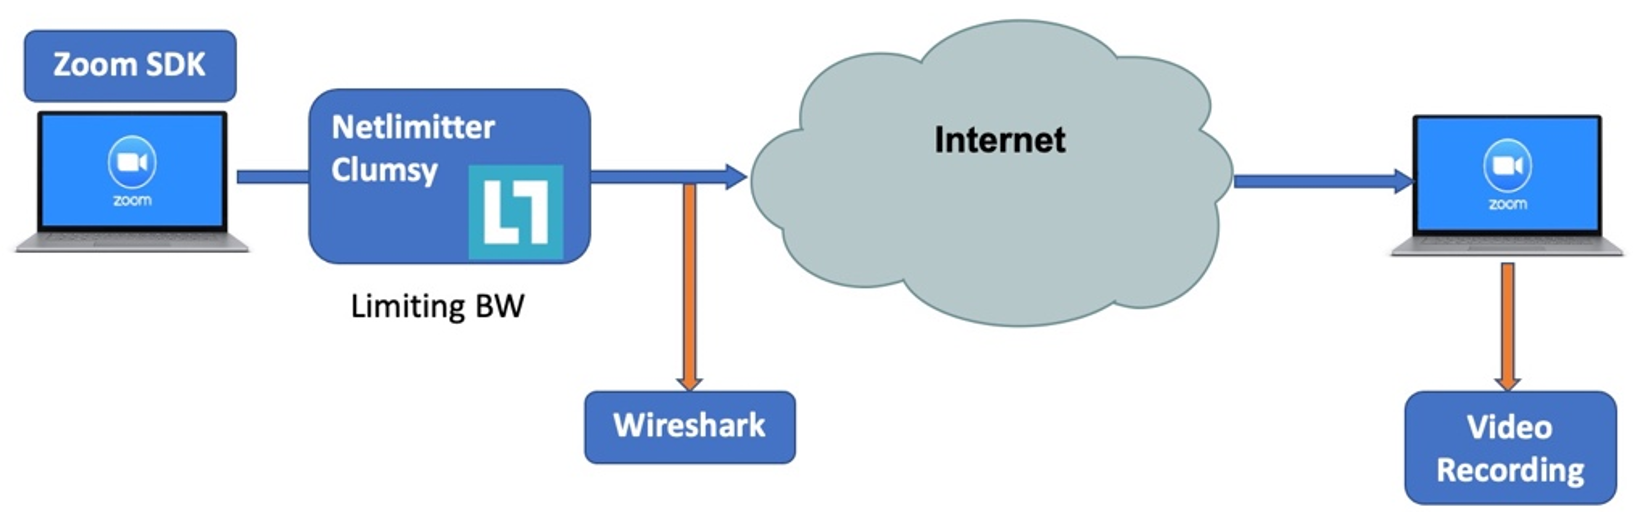
\includegraphics[scale=0.18]{exp_setup.png}
    \caption{Setup used to capture Zoom traffic features and labels}
    \label{fig:exp-setup}
\end{figure}


\section{Zoom Video Conferencing Behaviour}
From the captured dataset we have infered the behaviour of the Zoom application, as a function of different channel conditions. We chose as the limittting parameter the bandwidth of the channel, as it is the easy to control, and also the easiest to interpret.
% While capturing the dataset of Zoom conferencing traffic samples, we have investigated Zoom behavior when exposed to varying channel bandwidth conditions. It is logical to assume that bandwidth transition periods will impact video quality and will reflect on users' perceived quality. Therefore, it is advantageous to understand the impact of these transitions on traffic features and labels.

\subsection{Impact of reduced available bandwidth}
We shall refer to 'transition' as the period during which the Zoom application adjusts its video transmission parameters when a degradation is introduced to the channel quality, such as a drop of bandwidth for example. We discovered that during transition, Zoom goes through the following cycle: (1) reducing video spatial resolution; (2) reducing frames per second (fps); and (3) restoring spatial resolution to original with lower fps. We observed that such a transition can typically take up to 10 sec, at the end of which the video spatial resolution is restored to the original value while a lower fps is used to compensate for the reduced available bandwidth. This behavior makes sense, given that in typical video conferencing scenario there are only small spatial movements and therefore users' perceived quality will be impacted more by the spatial resolution than by the temporal resolution. The charts of \Cref{fig:adapt-patt} illustrate the steady state variation of fps and latency as a function of available bandwidth (measured after waiting for the transition period to pass and the spatial resolution to be restored). They were taken from a single session; however, they represent a consistent behavior that we have observed in multiple similar sessions. A dramatic drop from 25 fps to less than 10 fps is observed when the available bandwidth drops from 120 kbps to 60 kbps. 
\subsection{Impact of reduced bandwidth on Quantization Parameter (Qp)}
Assuming that Qp may be used by Zoom as a dominant parameter to adapt to changing channel bandwidth conditions, and therefore may be used as a good indicator for QoE, we have explored the change of Qp when reducing the available bandwidth. We observed that the Qp remains unchanged for I-frames and is slightly decreased with reduced bandwidth for P-Frames. This indicates that the Zoom application tries to compensate for the reduced bandwidth, which is accommodated by reduced fps, by adjusting to finer quantization of the P-Frames, however, the change is small, and we consider it too hard to estimate from encrypted traffic. Therefore, it is less valuable as QoE predictor. The change of Qp with the reduced bandwidth is illustrated in \Cref{fig:qp-change}.

\begin{figure}
    \centering
    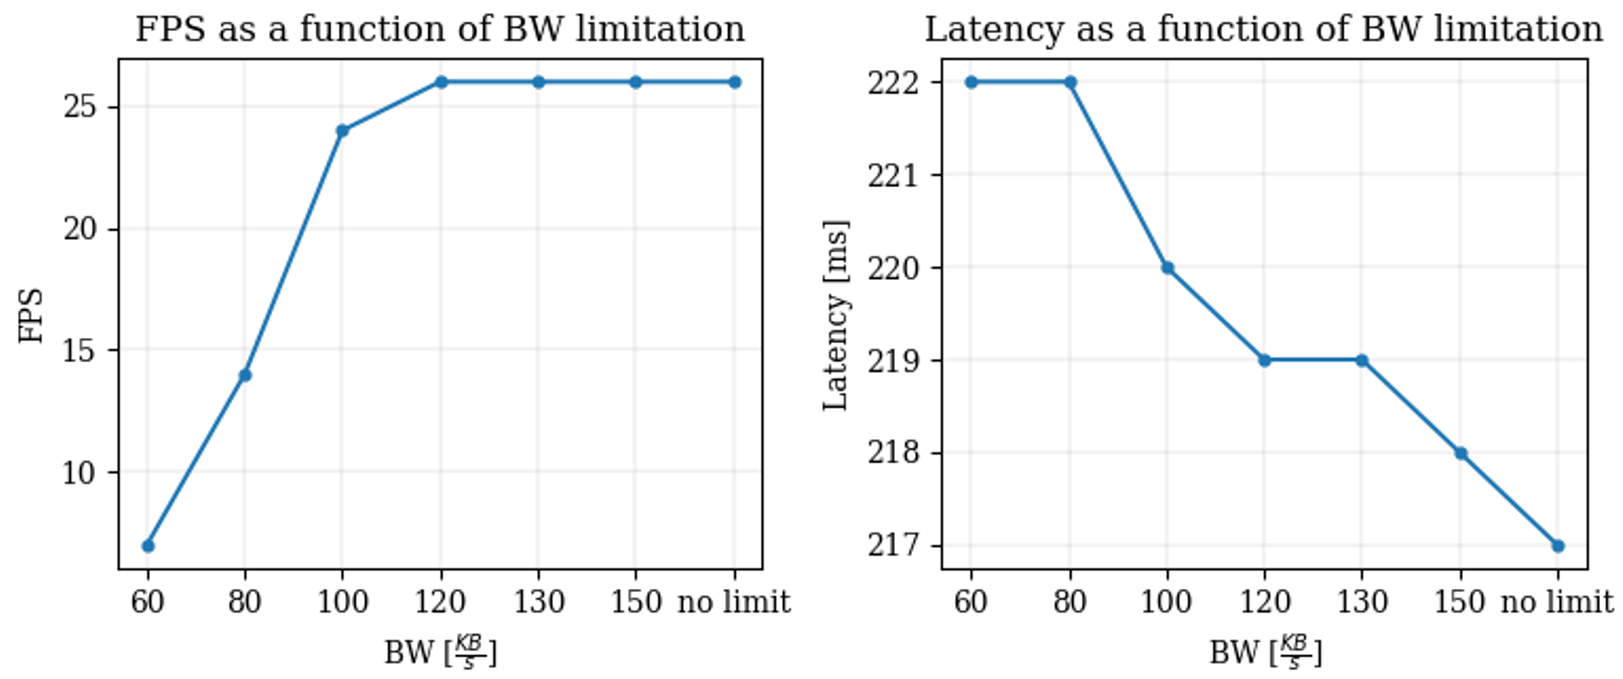
\includegraphics[scale=0.18]{adapt_patt.png}
    \caption{Zoom adaptation patterns to dropping bandwidth}
    \label{fig:adapt-patt}
\end{figure}

\begin{figure}
    \centering
    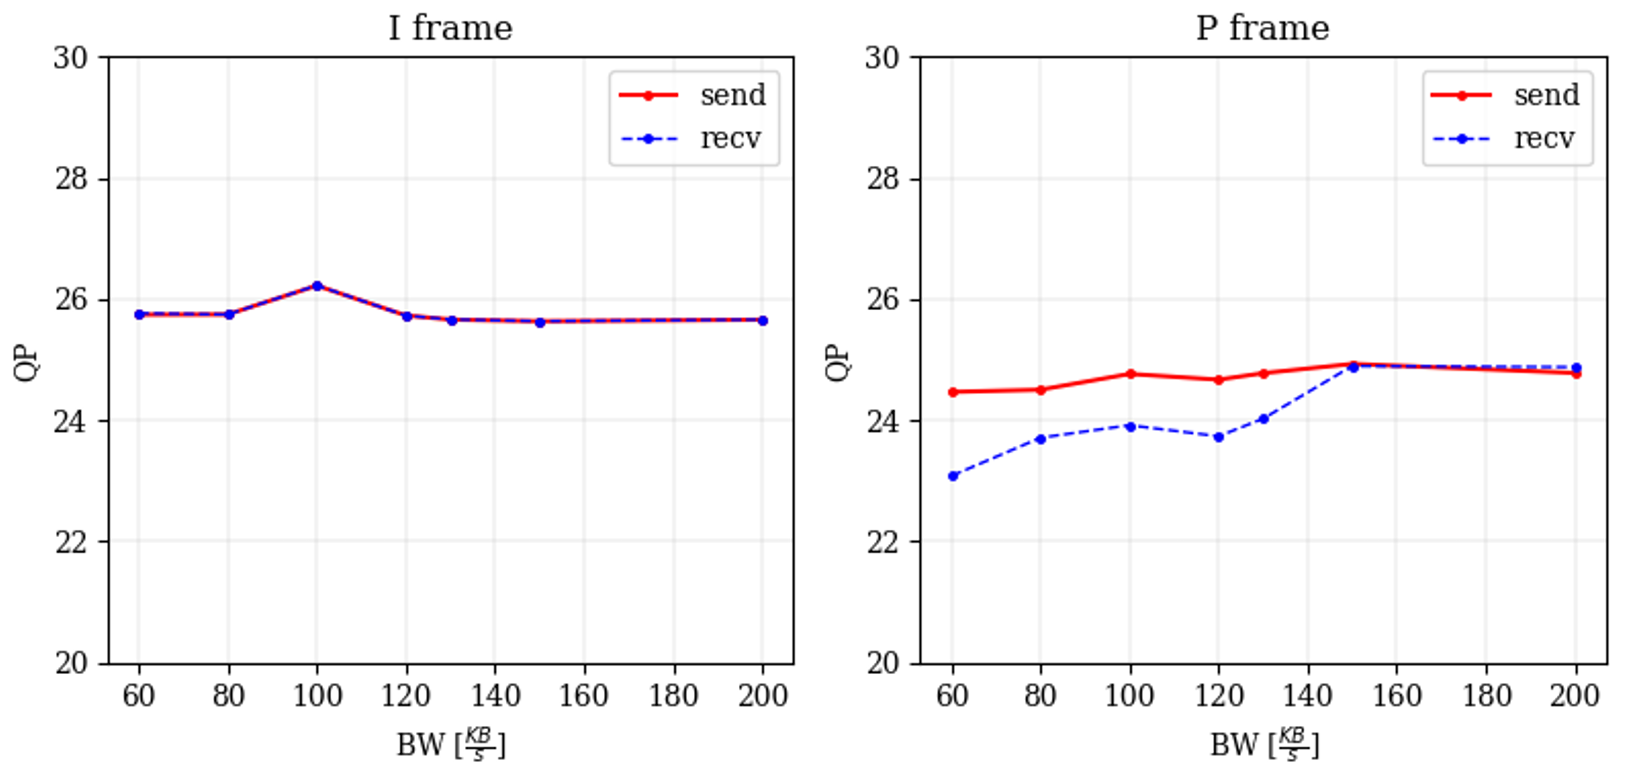
\includegraphics[scale=0.18]{Qp_to_bw.png}
    \caption{Zoom Qp change as a function of dropping bandwidth}
    \label{fig:qp-change}
\end{figure}

% \subsection{Full Reference (FR) QoE metrics}
% We extracted several Full Reference video quality metrics from Zoom traffic. In order to assess the quality degradation caused by reduced bandwidths, we needed to compare a reference source video of original quality to the same video stream at the receiving end, that was impacted by the network conditions. We have access to the video that is recorded by the Zoom application. We observed that when establishing a 2-party conference call, Zoom reduces the quality of the recoded video at the source and at the destination at the same time. In order to obtain a good quality reference, we managed to force the Zoom application to produce and record a good quality video. This was accomplished by adding to the call a 3rd party without a bandwidth limitation. This way the sending Zoom application allows to record a good quality reference which is not impacted by the restricted bandwidth of the 2nd party to the call. The setup used to record the reference and the destination videos is depicted in \Cref{fig:vmaf-setup}. In order to perform a reasonably accurate comparison between the 2 recorded streams, they have to be synchronized. We used the audio recording to synchronize the streams by creating an abrupt loud instantaneous noise (similar to "cut" used in recording a movie "video take") and synchronized the videos at the sender and recipient ends using that noise.
% The results of the Full reference video QoE metrics measured using the setup depicted in \Cref{fig:vmaf-setup} are provided in \Cref{fig:qual-metrics}. The slight improvement of quality observed when the bandwidth is decreased can be explained by the slight decrease of the Qp parameter performed by Zoom during the bandwidth drop transition period (depicted in \Cref{fig:adapt-patt}). It is assumed that Zoom decreases the Qp to compensate for reduced quality during the bandwidth drop transition.

\begin{figure}
    \centering
    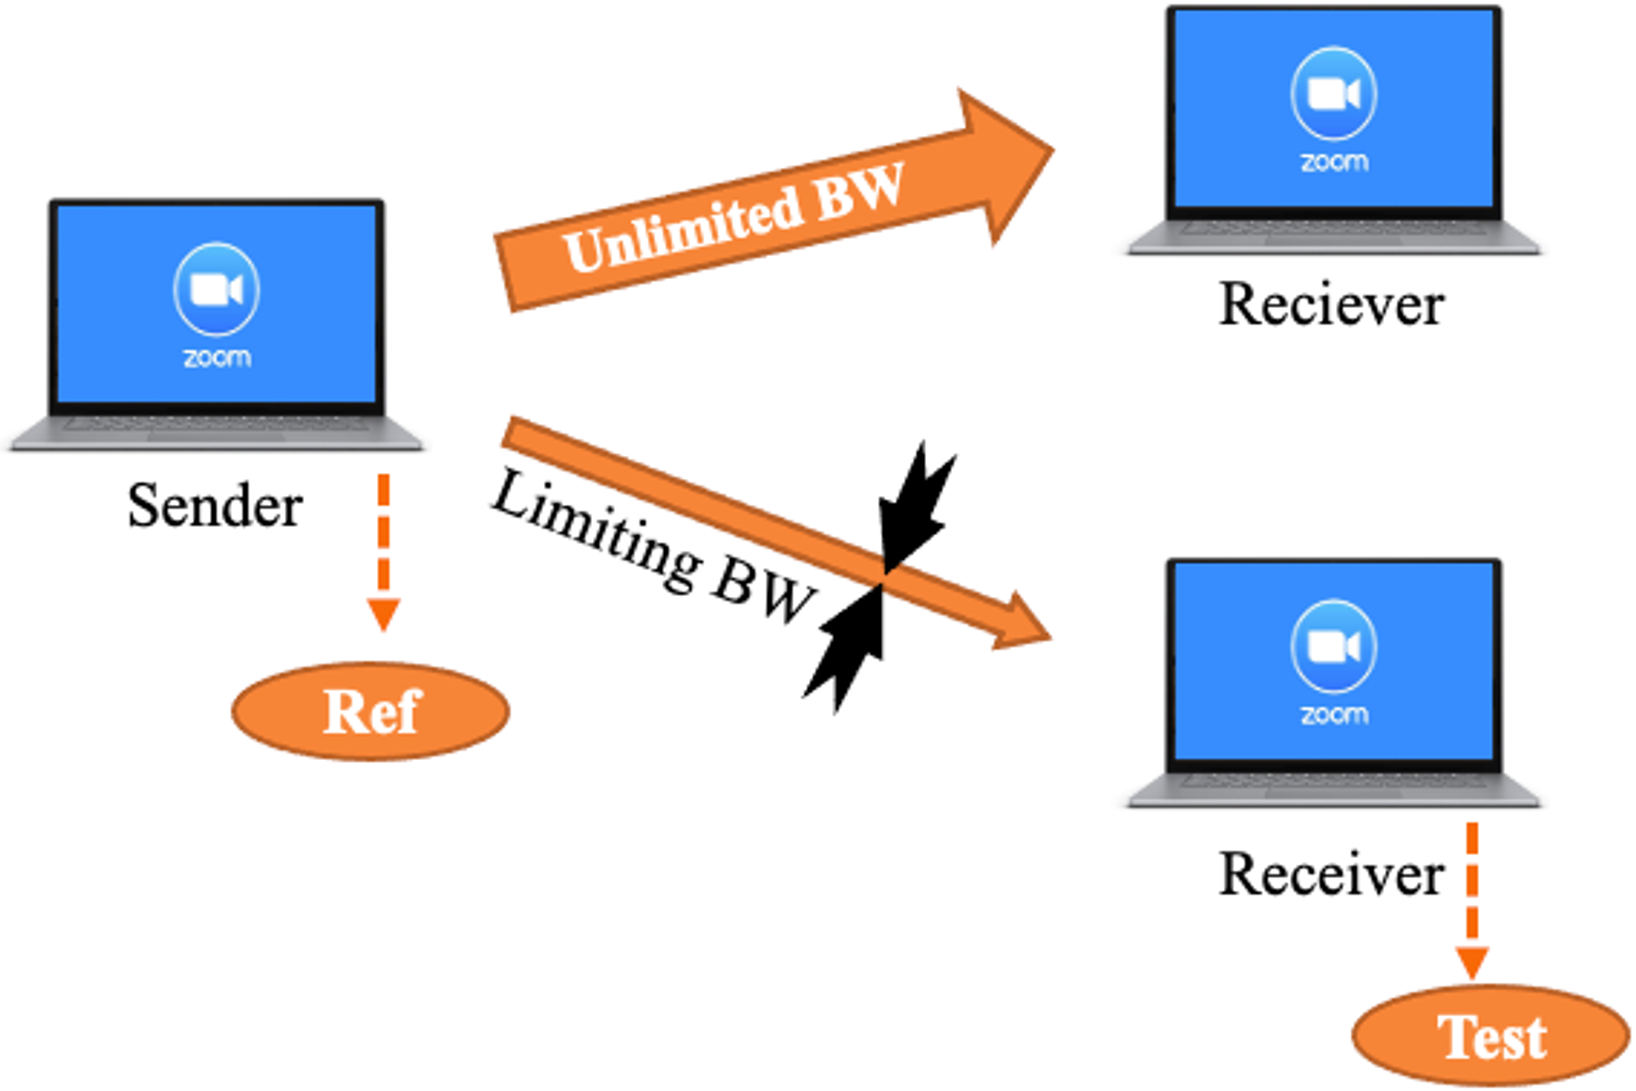
\includegraphics[scale=0.18]{vmaf_setup.png}
    \caption{VMAF full reference Zoom testing setup}
    \label{fig:vmaf-setup}
\end{figure}

\begin{figure}
    \centering
    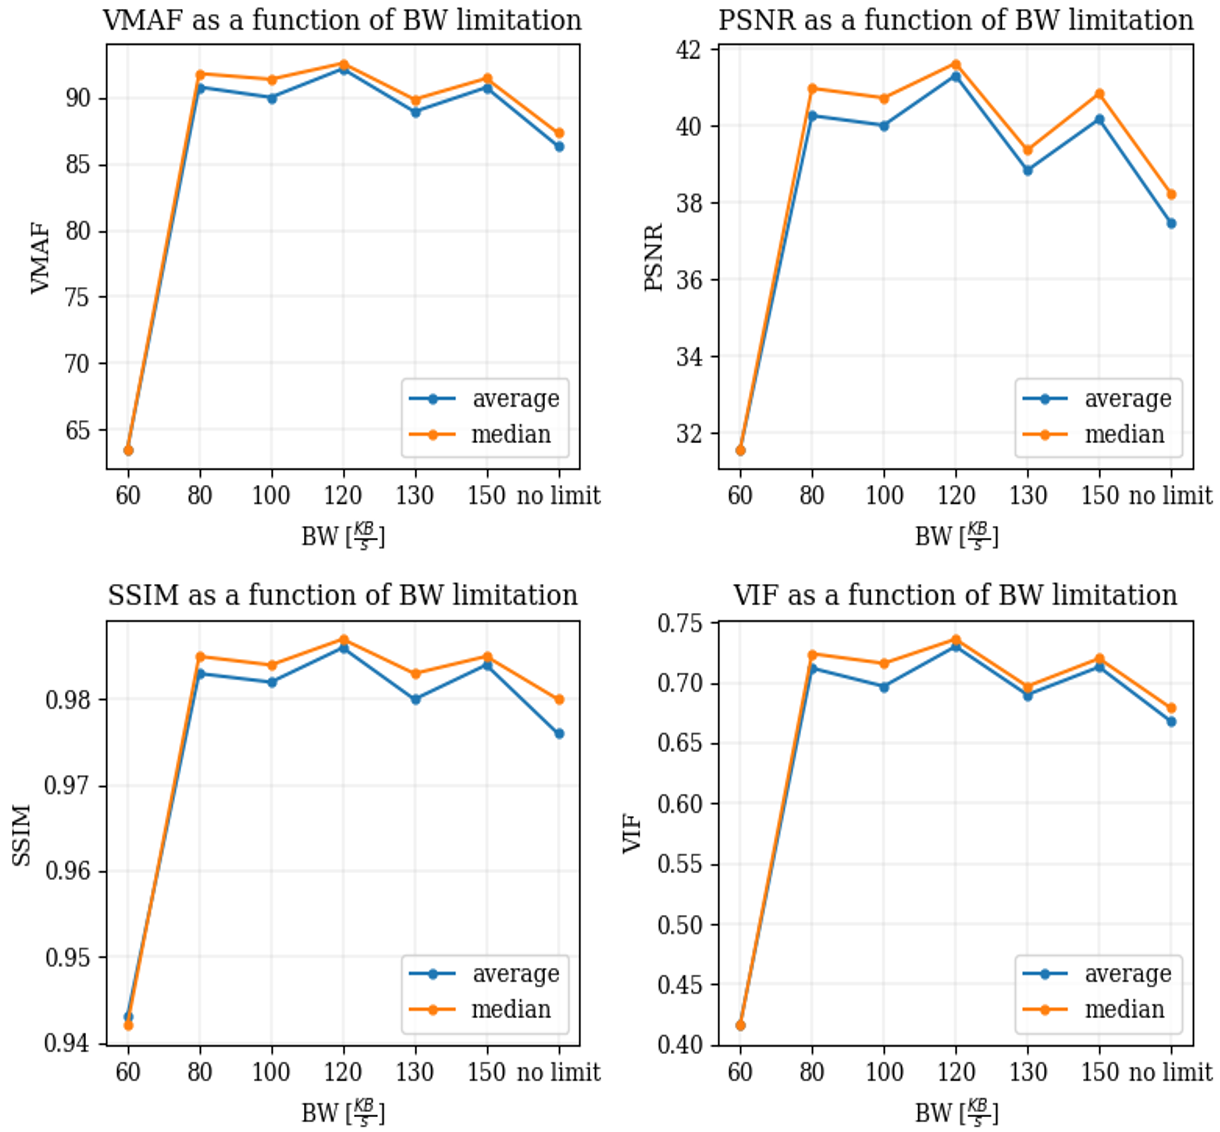
\includegraphics[scale=0.25]{vmaf_to_bw.png}
    \caption{Measured Zoom quality metrics as a function of dropping bandwidth}
    \label{fig:qual-metrics}
\end{figure}


% \subsection{NIQE – NR quality metric}
% Due to the challenges of recording Zoom video sessions with FR and in order to make the dataset more accommodating to future expansions (which do not necessitate complicate setups and saving of a refence for each recorded video clip), we researched the No Reference (NR) QoE metric alternatives. A promising NR metric that has emerged is the Naturalness Image Quality Evaluator (NIQE) \cite{mittal2012making}, which measures the distance of the frame from naturalness, therefore, a smaller score indicates better perceptual quality. NIQE measures the distance between the Natural Scene Statistics (NSS)-based features calculated from an image to the features obtained from an image database used to train the model. The features are modeled as multidimensional Gaussian distributions. We calculated NIQE as a function of bandwidth, resolution and fps. The corresponding graphs are depicted in \Cref{fig:niqe-fps-bw-res}. As can be seen in \Cref{fig:niqe-fps-bw-res} (b) and (c), the NIQE is consistent with available bandwidth and video frame resolution respectively, such that the larger the bandwidth or the resolution, the smaller the NIQE, thus indicating better quality.  We can observe a range of resolutions for which the NIQE value remains constant, indicating that the image naturalness metric at these resolutions is sufficiently good despite the change. An interesting observation is depicted in \Cref{fig:niqe-fps-bw-res} (a), indicating a change of NIQE with fps, whereas the metric is measured per single frame and is therefore spatial by nature. The temporal resolution of the video frames has an impact on the spatial quality. This is due to the compression algorithm that utilizes quantized residuals which are determined by block prediction accuracy, which is in turn impacted by the magnitude of the Motion Vectors (MV) used for Inter-prediction. The larger the movement between consecutive frames, the larger the MV magnitude and the less accurate is the prediction, thus increasing the value of the temporary predicted block residuals and reducing the quality due to their quantization.

\begin{figure}
    \centering
    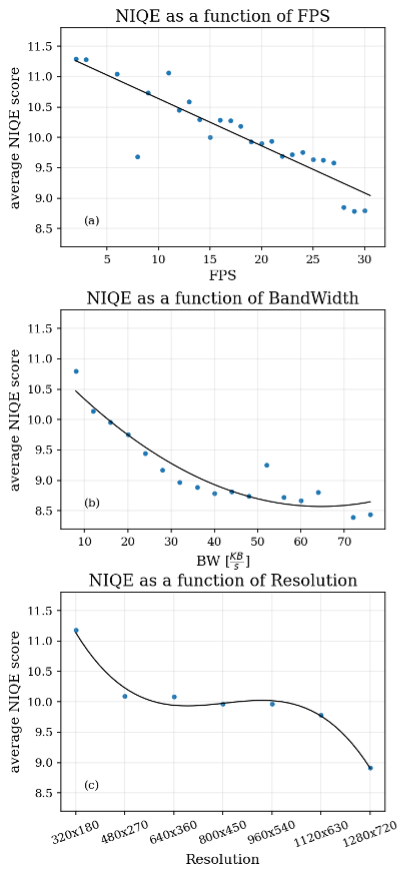
\includegraphics{niqe_to_fps.png}
    \caption{Measured Zoom NIQE quality metric as a function of fps, bandwidth, and resolution}
    \label{fig:niqe-fps-bw-res}
\end{figure}
\section{Results} 
Decision trees emerge as the most accurate ML algorithm for classifying encrypted VoD traffic \cite{orsolic2018youtube} \cite{dimopoulos2016measuring} \cite{orsolic2017machine}. We used a Decision Tree model to predict video spatial resolution. The different spatial resolution labels that have been observed are: 1280x720, 1120x630, 960x540, 800x450, 640x360, 480x270, and 320x180. We used the Gini \cite{gini1936measure} index as a classification criterion. It measures the split quality - let the data at node m be represented by $Q_m$ with $N_m$ samples, let the target be a classification outcome with possible values $0, 1, …., K-1$, then for node m, let the term of \cref{eq:pm} be the proportion of class k observations in node m. If m is a terminal node, predicted probability for this region is set to $p_{mk}$. And the measure of impurity is represented by \cref{eq:hqm}. We used best split as the splitter strategy at each node.

\begin{equation}
    p_{mk} = \frac{1}{N_m}\sum_{y \in Q_m}I(y=k)
    \label{eq:pm}
\end{equation}

\begin{equation}
    H(Q_m) = \sum_k p_{mk}(1-p_{mk})
    \label{eq:hqm}
\end{equation}
We further calculated Permutation Feature Importance, to understand which features are more dominant for the QoE prediction. Permutation Feature Importance provides a score for each feature, whereas the highest the score, the more relevant the feature is for predicting the output label. The permutation feature importance is a model agnostic approach, calculated by noticing the increase or decrease in error when we permute the values of a feature. If permuting the values cause a huge change in the error, it means the feature is important for our model. The permutation feature importance is based on an algorithm that works as follows: (1) Calculate the mean squared error between the model results and the known labels with the original values; (2) Permute the values for the features and make predictions again; (3) Calculate the mean squared error with the shuffled values; (4) Compare the difference between them; (5) Sort the differences in descending order to get features with most to least importance.
The results are depicted in \Cref{fig:feat-import} and indicate that the bandwidth (Bits Per Second) represents the most dominant feature but Packet Length and Average Time Between Packets fall not far behind.
To gain better understanding of the features and their impact on the classification result, we performed a correlation check between the three most dominant features. As can be seen in \Cref{fig:feat-corr}, the correlation between the three dominant features is high, so we can conclude that the most applicable feature is the bandwidth. We used a Decision Tree model for classification of the video resolution. The rest of the QoE labels – fps, NIQE, Latency and Jitter are represented by integer values, which are more suitable for regression. We compared the results of a regression algorithm to those of Artificial Neural Network and found the later to be more accurate. The accuracy of our results is provided in \cref{tab:final_accuracy}. The network was created using the "Sequential" module of the Keras library. The used fully connected network is depicted in \Cref{fig:nn-arch}.
For the regression network we have used the ReLU activation function, batch size 20, and 50 Epochs. We used the 'Adam' optimizer.
The accuracy was calculated by applying the trained model to each row of testing dataset (30\% of the data samples) as the Absolute Percentage Error. We calculated the average of all the rows to obtain the Mean Absolute Percentage Error (MAPE). We further calculated Permutation Feature Importance, to understand which features are more dominant for the QoE prediction. Permutation Feature Importance provides a score for each feature, whereas the highest the score, the more relevant the feature is for predicting the output label. The permutation feature importance is a model agnostic approach, calculated by noticing the increase or decrease in error when we permute the values of a feature. If permuting the values cause a huge change in the error, it means the feature is important for our model. The permutation feature importance is based on an algorithm that works as follows: (1) Calculate the mean squared error between the model results and the known labels with the original values; (2) Permute the values for the features and make predictions again; (3) Calculate the mean squared error with the shuffled values; (4) Compare the difference between them; (5)	Sort the differences in descending order to get features with most to least importance.
The results are depicted in \Cref{fig:feat-import} and indicate that the bandwidth (Bits Per Second) represents the most dominant feature but Packet Length and Average Time Between Packets fall not far behind.

\begin{figure}
    \centering
    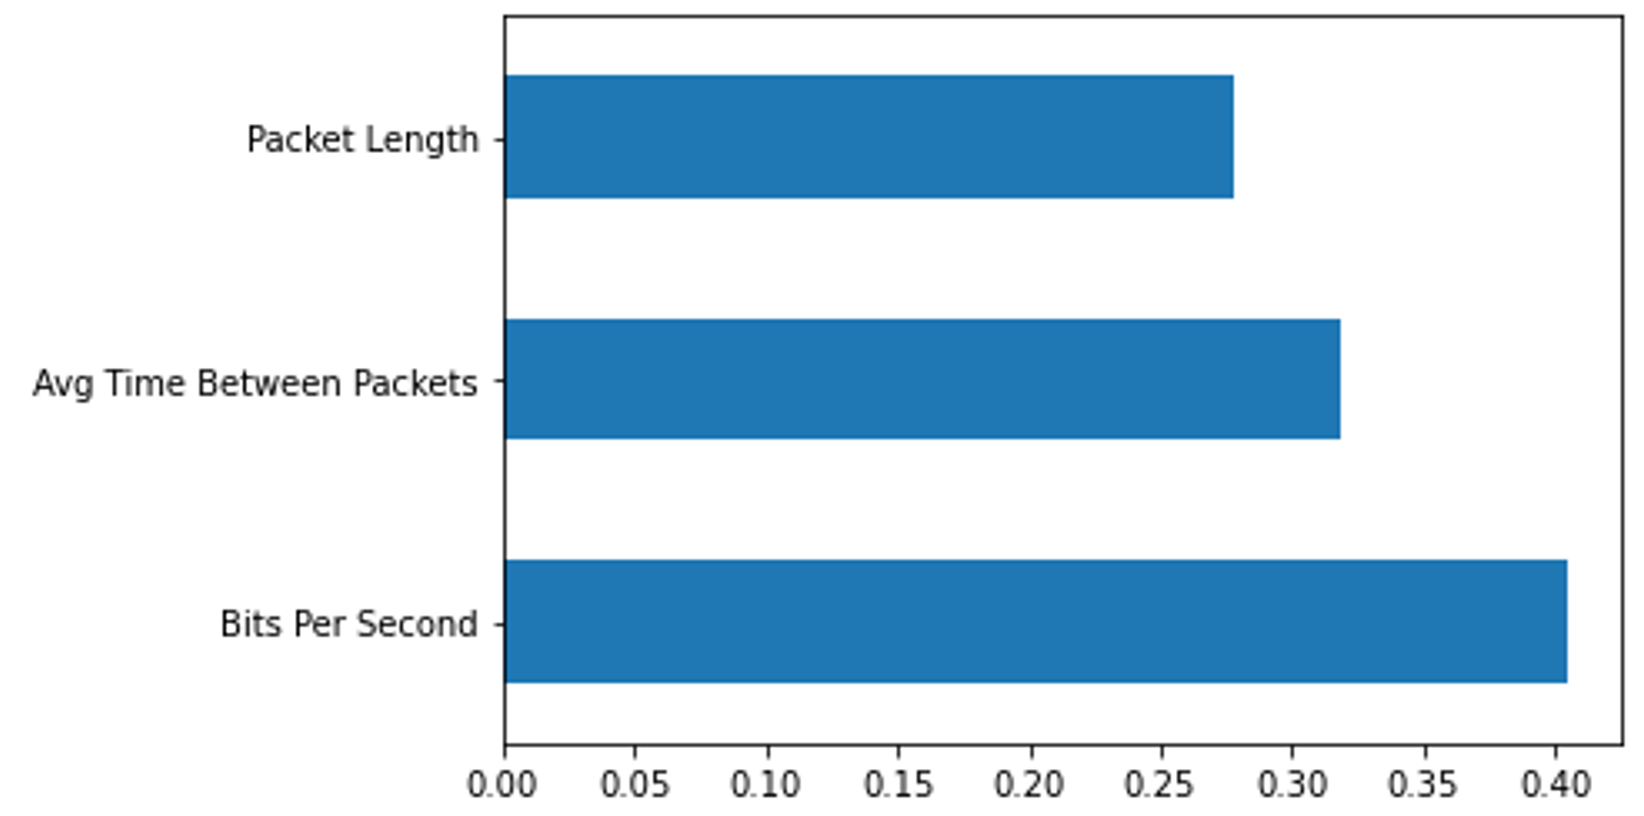
\includegraphics[scale=0.18]{feat_import.png}
    \caption{Feature importance calculation}
    \label{fig:feat-import}
\end{figure}

To gain better understanding of the features and their impact on the classification result, we performed a correlation check between the three most dominant features. As can be seen in \Cref{fig:feat-corr}, the correlation between the three dominant features is high, so we can conclude that the most applicable feature is the bandwidth. We used a Decision Tree model for classification of the video resolution. 

We trained a deep neural network with 16-64 layers and 128-256 units in each layer, as shown in \cref{fig:nn-arch}. We split the data into train and test dataset with a proportion of 90:10\%, while the train data was further split each train procedure with proportion of 80:20\% for the train data and validation respectively to monitor the performance in the course of the training. 
Parameter selection was done by a 5-fold cross validation where each time the train and test data was chosen anew in a non-overlapping manner (i.e., the tests of all the 5 folds were cohosen as non-overlapping sets).
The performance of the NN are summarized in \cref{tab:ablation}, for each of the predicted labels, viz. NIQE, Resolution and FPS.
% The rest of the QoE labels – fps, NIQE, Latency and Jitter are represented by integer values, which are more suitable for regression. We compared the results of a regression algorithm to those of Artificial Neural Network and found the later to be more accurate. 
% The accuracy of our results is provided in Table 1. The network was created using the "Sequential" module of the Keras library. The used fully connected network is depicted in \Cref{fig:nn-arch}.
% For the regression network we have used the ReLU activation function, batch size 20, and 50 Epochs. We used the 'Adam' optimizer.
% The accuracy was calculated by applying the trained model to each row of testing dataset (30\% of the data samples) as the Absolute Percentage Error. We calculated the average of all the rows to obtain the Mean Absolute Percentage Error (MAPE).

\begin{table}[]
    \centering
    \caption{QoE prediction accuracy results}
    \begin{tabular}{l|l|c}
        Predicted Label & Model & Accuracy \\
        \hline
        Resolution & DT & 90.489\% \\
        FPS & NN & 92.492\% \\
        NIQE & NN & 97.643\% \\

    \end{tabular}
    \label{tab:final_accuracy}
\end{table}

\begin{figure}
    \centering
    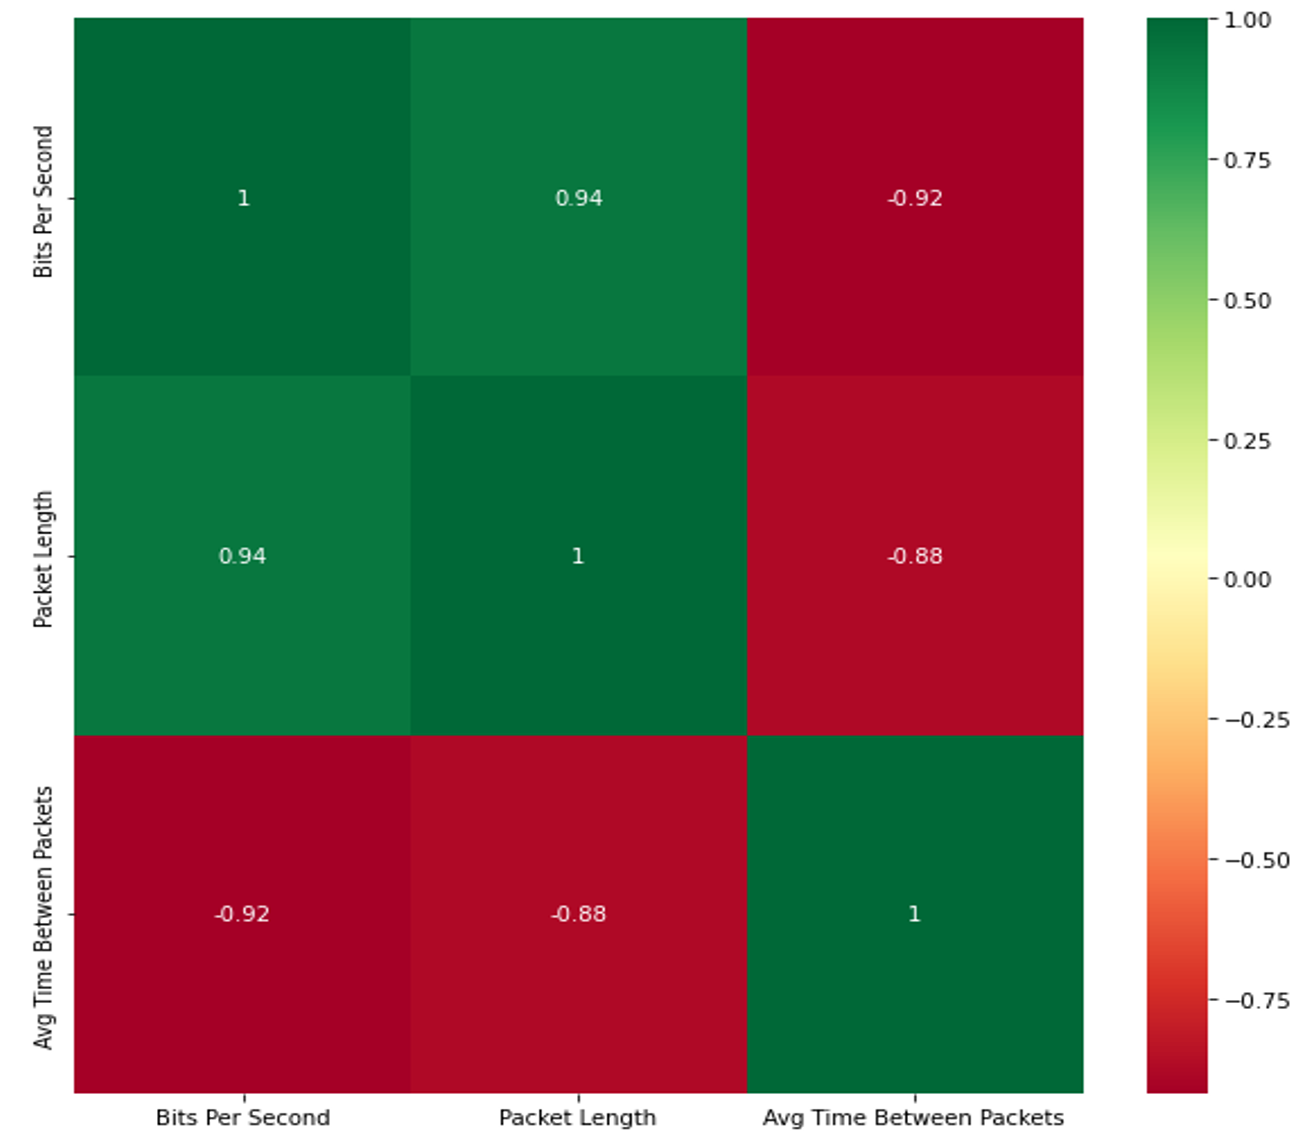
\includegraphics[scale=0.25]{conf_mat.png}
    \caption{Correlation between features}
    \label{fig:feat-corr}
\end{figure}

\begin{figure*}
    \centering
    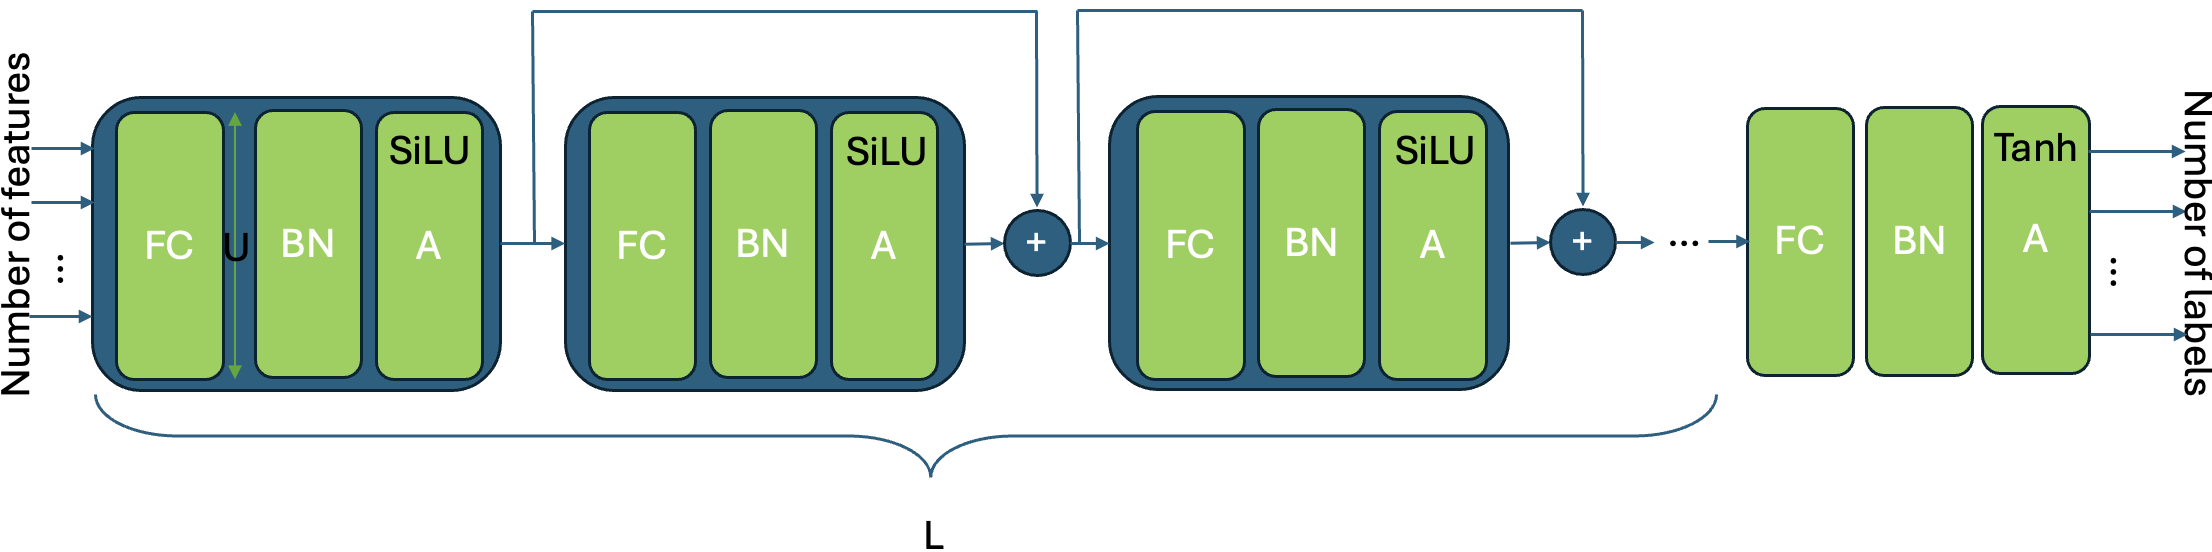
\includegraphics[scale=0.45]{figures/QNN Design.png}
    \caption{QoE prediction Neural Network architecture}
    \label{fig:nn-arch}
\end{figure*}
\section{Ablation Study}
We used the parameters $\mathbb{L}$ and $\mathbb{N}$ as the number of layers and units in each layer respectively. To find the best parameters for the NN, we divided the data in 70:20:10 ration for train, validation and test data respectively, where the train and validation datasets were determined randomly each execution, while the test set was randomly chosen, and set aside for an unbiased test evaluation. 

We performed the experiments on $\mathbb{L} \in \{2, 4, 8, 16, 32\}$ and $\mathbb{U} \in \{4, 8, 16, 32, 64, 128, 256\}$, and the corresponding results are listed in \cref{tab:ablation}. For networks with $\mathbb{L} > 8$ we employed skip connections as in \cite{he2016deep}.

\begin{table*}[]
\centering
        \begin{tabular}{|c|c|c|c|c|c|c|c|c|}
                \hline
                \makecell[l]{Train\\Epochs} & \makecell[l]{Number of\\Layers} &  \makecell[l]{Number of\\Units} & \makecell[l]{Initial\\Learning\\Rate} & \makecell[l]{Trainable\\Parameters} & NIQE & Resolution & \makecell[l]{Frames per\\Second\\(FPS)}\\
                \hline
                \multirow{3}*{10}  & 32 & 128 & 0.002 & 537865  & \textbf{2.746} & 11.619          & 8.692\\
                                   \cline{2-8}
                                   & 64 & 64  & 0.001 & 275081  & 3.192          & \textbf{10.257} & 10.496\\
                                   \cline{2-8}
                                   & 16 & 64  & 0.001 & 69257   & 3.015          & 11.285          & \textbf{7.541}\\
                                 
                \hline
                \multirow{3}*{50}  & 32 & 256 & 0.01 & 2124297  & \textbf{2.357} & 11.448          & 8.028\\
                                   \cline{2-8}
                                   & 32 & 128 & 0.008 & 537865  & 2.876          & \textbf{9.511}  & 10.605\\
                                   \cline{2-8}
                                   & 64 & 256 & 0.002 & 4246025 & 2.738          & 10.236          & \textbf{7.508}\\
                \hline
                \multirow{3}*{100} & 32 & 128 & 0.01  & 537865  & \textbf{2.395} & 11.268          & 8.810\\
                                   \cline{2-8}
                                   & 64 & 128 & 0.01  & 1074441 & 2.831          & \textbf{9.764}  & 10.272\\
                                   \cline{2-8}
                                   & 16 & 256 & 0.01 & 1063433  & 2.778          & 10.585          & \textbf{7.523}\\
                \hline
   
        \end{tabular}
    \caption{Parameter selection with 5-fold cross validation, and Adam optimizer set to default parameters, except initial learning rate. In bold face are the best result for each of NIQE, Resolution and FPS}
    \label{tab:ablation}
\end{table*}
\section{Conclusions and Future Work}
We have explored the extraction of QoE metrics of encrypted Zoom video conferencing traffic. By using Decision Tree algorithms, which have emerged as a predominant classification method for VoD traffic, we have obtained similar accuracy results for classifying resolution on our relatively small dataset of 720 samples. We further used a Neural Network model to predict additional QoE metrics that were extracted from the Zoom application and calculated from the video streams themselves. We have demonstrated excellent accuracy in predicting the Naturalness Image Quality Evaluator (NIQE). We are presently working on enhanced automations that will allow us to capture larger datasets in order to drive a more robust and generic prediction model. In addition, we plan to expand the scope of this research to other video conferencing tools, notably Microsoft Teams and Google GoToMeeting. We further plan to create a large dataset of Video Conferencing clips and perform a Mean Opinion Score (MOS) experiment with human observers. We will then compare the results of the metrics to those of the MOS and perform classification for both. 
\section{Acknowledgments}
We thank undergrad students for their diligent contribution to this paper: Sharon Golkarov, Yogev Drori, Nadav Hadad, Tamir Cohen, Max Polnikov, Or Shamir.

\printbibliography

\end{document}
